\documentclass{jlreq}

\usepackage{bm}
\usepackage{fancyhdr}
\usepackage{float}
\usepackage{graphicx}
\usepackage{listings}

\lstset{
    language=C, % 使用するプログラム言語を指定
    basicstyle=\ttfamily\footnotesize, % フォントの指定
    numbers=left, % 行番号を表示(必要な場合)
    numberstyle=\tiny, % 行番号のスタイル
    frame=single, % ソースコードを枠で囲む(必要な場合)
    breaklines=true, % 長い行を自動的に折り返す
    captionpos=b, % キャプションの位置を下にする
    showstringspaces=false, % 文字列内のスペースを表示しない
    keywordstyle=\color{blue}, % キーワードの色
    commentstyle=\color{green}, % コメントの色
    stringstyle=\color{red}, % 文字列の色
}
\renewcommand{\lstlistingname}{ソースコード}

\pagestyle{fancy}
\fancyhf{}
\fancyhead[R]{\thepage}

\renewcommand\thesubsection{(\alph{subsection})}

\title{言語処理プログラミング 課題2}
\author{22122502 川口 栄宗}
\date{提出日: \today}

\begin{document}

\maketitle
\clearpage

\section{作成したプログラムの設計情報}

\subsection{全体構成}

\subsection{各モジュールごとの構成}

\section{テスト情報}

\subsection{テストデータ}
\subsubsection{ブラックボックステスト}
ブラックボックステストには用意されていたテストデータを用いた.テストデータを以下に示す.
\begin{itemize}
  \item sample11.mpl
  \item sample011.mpl
  \item sample11p.mpl
  \item sample11pp.mpl
  \item sample12.mpl
  \item sample012.mpl
  \item sample12cr.mpl
  \item sample12crlf.mpl
  \item sample012eof.mpl
  \item sample12lf.mpl
  \item sample12lfcr.mpl
  \item sample012n.mpl
  \item sample012neof.mpl
  \item sample012s.mpl
  \item sample012seof.mpl
  \item sample13.mpl
  \item sample013.mpl
  \item sample14.mpl
  \item sample014.mpl
  \item sample014a.mpl
  \item sample014b.mpl
  \item sample14p.mpl
  \item sample15.mpl
  \item sample15a.mpl
  \item sample16.mpl
  \item sample17.mpl
  \item sample18.mpl
  \item sample19p.mpl
\end{itemize}

\subsubsection{ホワイトボックステスト}
ブラックボックステストに用いたデータと同じものを用いた.

\subsection{テスト結果}
\subsubsection{ブラックボックステスト}
docker環境でのブラックボックステストの結果を図\ref{fig:black_box_test}に示す.
\begin{figure}[H]
  \centering
  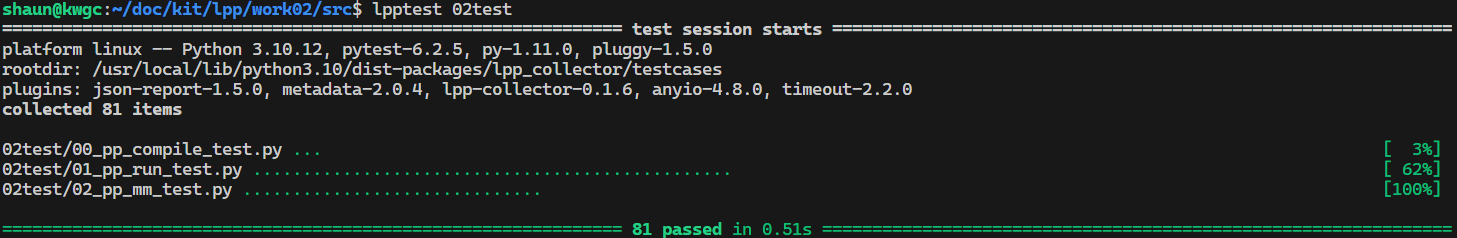
\includegraphics[width=\textwidth]{assets/black_box_test.png}
  \caption{ブラックボックステストの結果}
  \label{fig:black_box_test}
\end{figure}

\subsection{ホワイトボックステスト}
ホワイトボックステストの結果を図\ref{fig:white_box_test}に示す.
\begin{figure}[H]
  \centering
  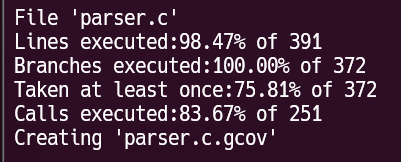
\includegraphics[width=\textwidth]{assets/white_box_test.png}
  \caption{ホワイトボックステストの結果}
  \label{fig:white_box_test}
\end{figure}

\subsection{テストデータの十分性}
ブラックボックステストでは,構文に関するテストや境界値のテストが含まれている.それらのテストが通ったことから,
外部仕様に関しては大きな問題は見られないと言える.

また,ホワイトボックステストでは未実装の拡張仕様については網羅率は$0\%$となっているが,字句解析を行うscan.cの命令網羅率は$91.95\%$と高い結果であった.

\section{課題のスケジュールと実際の進捗状況}
\subsection{事前計画}
\begin{figure}[H]
  \centering
  \includegraphics[width=\textwidth]{assets/schedule_01.png}
  \caption{課題1の事前のスケジュール}
  \label{fig:schedule01_pre}
\end{figure}

\subsection{実際の進捗状況}
\begin{table}[H]
  \centering
  \caption{課題1の実際の進捗}
  \scalebox{0.6}{
    \begin{tabular}{cccc}
      \hline
      開始日 & 終了日 & 取り組み時間 & 作業内容                                                                                                       \\ \hline
      10/3   & 10/16  & 3            & 資料を読んで仕様をまとめ,概略設計を行う                                                                       \\
      10/16  & 10/26  & 3            & トークンカウント用の配列初期化とスキャナを用いたトークンカウント部の作成,またカウントした結果の出力部分の完成 \\
      10/26  & 12/16  & 8            & スキャナの作成                                                                                                 \\
      10/26  & 12/16  & 2            & テスト工程                                                                                                     \\
      12/16  & 1/8    & 6            & レポート作成                                                                                                   \\
      \hline
    \end{tabular}
  }
\end{table}

\subsection{当初の事前計画と実際の進捗との差の原因}
10月中に課題1を終わらせる予定であったが,同時並行して進めていたハッカソンや就活に重きをおいてしまい,本課題に支障が出てしまった.
その後も中途半端にスケジュールを詰めたことにより,課題の進捗を生めなかった.課題1の難易度を甘く見積もっており,優先順位を後回しにしたことにより
本課題の進捗の遅延や,他実験のレポートや就活との渋滞に繋がってしまった.これらは,適切にスケジュールを組み,日ごろからチェックすることで
遅延は回避できた可能性がある.

\end{document}